\documentclass[12pt]{article} % Define document class
%\usepackage{amsmath} % ?
\usepackage{graphicx} % Need for images
%\usepackage{float}% ??
%\usepackage[font={small,it}]{caption}
%\pagenumbering{arabic}

\graphicspath{{./img/}} % Define graphics path for graphicx

% Hyperlinks in PDF:
\usepackage{hyperref, color}
\definecolor{linkcolor}{rgb}{0,0,0.4}
\hypersetup{
		breaklinks=true,
		colorlinks=true,
		linkcolor=linkcolor,
		urlcolor=linkcolor,
		citecolor=black,
		filecolor=black,
		%filecolor=blue,
		pdfmenubar=true,
		pdftoolbar=true,
		bookmarksdepth=3   % Uncomment (and tweak) for PDF bookmarks with more levels than the TOC
	    }

%https://www.sharelatex.com/blog/2012/01/31/keep-track-of-your-labels-with-showlabels.html	    
%\usepackage[inline]{showlabels} % doesn't work with amsmath labels
\usepackage{amsmath} % For referencing eq with \eqref (showing numbers) insted of /ref

\begin{document}
\title{Project 3: Ordinary Differential Equations and the Solar System}
\author{Michael Saybolt \\ Bjon Charlery}

%	\date{\today}
\date{5/2/2017}
\maketitle
\pagebreak

\tableofcontents

\begin{abstract}
This project explored a model of the solar system created by solving Ordinary Differential Equations (ODE). Numerical integration was done using the Euler method, as well as a Verlet method. In addition, emphasis was placed on object orienting the code for modularity, and continuously testing as the code is developed to stop bugs before they grow or are harder to find.
\end{abstract}

\pagebreak % A page break
%\bigskip
%\bigskip

\section{Introduction} % Shows how to use a link
\indent The objective of this project was to solve coupled differential equations responsible for the trajectory of planets around the solar system. Initial conditions for the solver were extracted from the following 
\href{{http://www.nasa.gov/index.html}}{NASA} 
website 
\href{{http://ssd.jpl.nasa.gov/horizons.cgi#top}}{\nolinkurl{http://ssd.jpl.nasa.gov/horizons.cgi\#top}}
.

%\indent The objective of this project was to solve a differential equation in the form of:\\ $$-u\textsuperscript{''}(x) = f(x), x\epsilon(0,1),u(0) = u(1) = 0.\\$$ that can be written into the linear equation $(Ax = b)$. Since A is a tridiagonal matrix there is an actual or analytical solution that can be made for this particular matrix. The following sections will describe the origins for the algorithms used and their respective results.
%

% Sentences can be broken up onto new lines, but skipping a line in the code does have an effect
For ease of debugging, a simulation of a simple binary system is created with just the Sun and the Earth.
The only force in the problem is gravity. Newton's law of gravitation  is given by a force $F_G$
\begin{equation} % MUST USE this format for eq number display wtf
%\[
F_G=\frac{GM_{\odot}M_{\mathrm{Earth}}}{r^2},
\label{eq:newtong}
%\]
\end{equation}
where $M_{\odot}$ is the mass of the Sun and $M_{\mathrm{Earth}}$ is the mass of the Earth. The gravitational constant is $G$ and $r$ is the distance between the Earth and the Sun. Eventually the other planets will be added, but for now just this system will be used to test the layout of the algorithms.


\section{Description}
%This section will detail the methods used to solve the linear equation system. It is solved using two methods:\\
%\begin{itemize}
%	\item \centering LU decomposition
%	\item \centering Tridiagonal Solver - Gauss Elimination\\
%\end{itemize}
This section will provide details about the general equations describing the sytem, and the general approach of the problem.

\subsection{Block tied to wall}
To refresh understanding of differential equations and how to code them, the block tied to a wall example was copied and analyzed.\\
Newton's equation of motion for system:
\[
m\frac{d^2x}{dt^2}=-kx,
\]
aka:
\[
\frac{d^2x}{dt^2}=-\frac{k}{m}x=-\omega_0^2x,
\label{eq:newton1}
\]
with the angular frequency $\omega_0^2=k/m$.
This DE has solutions that can be obtained analytically of the form
\[
	x(t)=Acos(\omega_0t+\nu),
\]
where $A$ is the amplitude and $\nu$ the phase constant.	

see line 1116 of ode.tex @Author: mhjensen for more equation

\subsection{Euler Method}
The Euler method is good for a quick and dirty way to see approximately what a solution looks like, at the expense of accuracy and numerical stability. There is also an enhanced Euler method, which offers better numerical stability that was not officially covered in this unit, but was discovered accidentally while making code. This is discussed later in the results setcion.

\subsection{Verlet Method: Velocity Verlet}
The Verlet method is another method of numerical integration, and offers good numeric stability thus is usually accurate. The Velocity Verlet method specifically is covered in this report, as that is the implementation chosen to solve this problem.

\section{Implementation}
This section will transform the equations described in the previous section into usable code, and also describe difficulties encountered, and implemented solutions.  For simplification in understanding, a 2D simplification of applying Newton's law of gravitation is studied. Recalling that Newton's law of gravitation is
\eqref{eq:newtong}, the position and velocity can be described by 4 coupled DEs:
\begin{equation}
	\frac{dv_x}{dt}=-\frac{GM_{\odot}}{r^3}x,
	\label{eq:simplea}
\end{equation}
\begin{equation}
	\frac{dx}{dt}=v_x,
	\label{eq:simplev}
\end{equation}
\[
	\frac{dv_y}{dt}=-\frac{GM_{\odot}}{r^3}y,
\]
\[
	\frac{dy}{dt}=v_y
\]

This would be the same for 1 or 3 dimensions. But,
\[
	GM_{\odot}=v^2r,
	\]

and assuming Earth's velocity is:
$v = 2\pi r/\mathrm{yr}=2\pi\mathrm{AU}/\mathrm{yr}$

Thus can equate the following for the acceleration in some (x) direction:

\begin{equation}
	\frac{dv_x}{dt} = -\frac{GM_{\odot}}{r^3}x = 4\pi^2 \frac{(\mathrm{AU})^3}{\mathrm{yr}^2}
	\label{eq:simplea2}
\end{equation}
replacing equation \eqref{eq:simplea}.

\subsection{Euler}
Descretizing the domain into timesteps \textit{h}, the Euler method describes the next step's position and velocity as:
\begin{equation}
	x_{i+1} = x_i + hv_i
	\label{eq:simplepeuler}
\end{equation}
\begin{equation}
	v_{i+1} = v_i - \frac{d(v_i)}{dt}
	\label{eq:simpleveuler}
\end{equation}

where \textit{x} signifies position, and \textit{v} signifies velocity in some direction at time step index \textit{i}.

The result of equation \eqref{eq:simplea2} can be substituted into \eqref{eq:simpleveuler}, resulting in

\begin{equation}	
	v_{i+1} = v_i - h(4\pi^2)\frac{x_i}{r_i^3}
	\label{eq:simpleveuler2}
\end{equation}
insert code

\subsubsection{Enhanced Euler}
The task for the Euler method was to use the regular Euler method. According to the notes, and equations \eqref{eq:simplepeuler} and \eqref{eq:simpleveuler}, which originate from the notes, or \eqref{eq:simpleveuler2}, the position and velocity are updated simultaneously.
Because code is sequential, the position must be stored before it is updated, so that it can be used in the velocity. But, discovered accidentally and observed in provided C++ implementation of the Euler method, if the value is not stored and the velocity is updated using the next iterations position, numeric stability is improved giving a more accurate solution. The C++ code should probably mention this distinction in my humble opinion.

This difference would make equation \eqref{eq:simpleveuler2} look like:
\begin{equation}	
	v_{i+1} = v_i - h(4\pi^2)\frac{x_{i+1}}{r_{i+1}^3}
\end{equation}
because position is updated before velocity when programmed, so without saving the 'old' position, the velocity actually contains the next iteration's position values.

\subsection{Velocity Verlet}
Descretizing the domain into timesteps \textit{h}, the Velocity Verlet method describes the next step's position and velocity as:
\begin{equation}
	x_{i+1} = x_i + hv_i + \frac{h^2}{2}\frac{dv_i}{dt}
	\label{eq:simpleposverlet}
\end{equation}
\begin{equation}
	v_{i+1} = v_i + \frac{h}{2}\left(\frac{d(v_{i+1})}{dt} + \frac{d(v_i)}{dt}\right)
	\label{eq:simplevverlet}
\end{equation}

As with the creation of the discretized Euler equations, equation \eqref{eq:simplea2} can be substituted into \eqref{eq:simpleposverlet} and \eqref{eq:simplevverlet}, resulting in
\begin{equation}
	x_{i+1} = x_i + hv_i + \frac{h^2}{2}\frac{-4\pi^2}{r_i^3}x_i
	\label{eq:simpleposverlet2}
\end{equation}
and
\begin{equation}
	v_{i+1} = v_i + \frac{h}{2}\left(\frac{-4\pi^2}{r_{i+1}^3}x_{i+1} + \frac{-4\pi^2}{r_i^3}x_i\right)
	\label{eq:simplevverlet2}
\end{equation}

Note that generating the next iteration's velocity requires the next iteration's position already, which complicates things, especially when introducing additional forces from other planets, not just the force of gravity from the Sun acting on earth.

\subsection{Adding Planets}
The previous equations describe the position and velocity of a planet in the next timestep for a binary system containing only the Earth and the Sun. Recall that the only force the orbiting planet experiences is from the gravity of the Sun, described by equation \eqref{eq:newtong}, thus giving equation \eqref{eq:simplea2}.

Adding additional planets changes the acceleration. Instead of the acceleration in some direction being described by equation \eqref{eq:simplea2}, it contains additional components from the gravity of the other planets acting upon it, and the other planets contain components of that planet's gravity, therefore each planet's acceleration contains a component of the force of gravity from the sun \textbf{and} a summation of the force of gravity from all other planets in the system, yielding:

%\[
%	\frac{dv_x}{dt} =  4\pi^2 \frac{(\mathrm{AU})^3}{\mathrm{yr}^2}
%]\

\begin{equation}
	\frac{dv}{dt} = \frac{-4\pi^2}{r^3}x + SUM(-4\pi^2\frac{\frac{mo}{m_{\odot}}}{rd^3}xd)
	\label{eq:moara}
\end{equation}
where $xd$ and $rd$ are the difference between the current planet and some other planet's position, and $md$ is the other planet's mass used in this summation of gravitational forces from all different planets, denoted as 'SUM'.
To better match the code, for this summation, the quantity $md$ (mass difference, or really a difference ratio) is assigned $\frac{mo}{m_{\odot}}$. Thus the acceleration of a planet due to the force of gravity from the sun and all other planets can be written as

\begin{equation}
	\frac{dv}{dt} = -4\pi^2(\frac{x}{r^3} + SUM(xd\frac{md}{rd^3})
	\label{eq:moara2}
\end{equation}

This modification to the previous substitution is integrated into the equation for the next time step's velocity in both the Euler and Verlet methods.

\subsubsection{Euler}
When doing the transformation shown by turning equation \eqref{eq:simpleveuler} into \eqref{eq:simpleveuler2} instead using equation \eqref{eq:moara2} containing gravity components from the other planets, the discretized velocity next iteration looks like
\begin{equation}
	v_{i+1} = v_i - h(4\pi^2)(\frac{x_i}{r_i^3} + SUM(xd_i\frac{md_i}{rd_i^3}))
	\label{moarveuler}
\end{equation}
instead of
\begin{equation}	
	v_{i+1} = v_i - h(4\pi^2)\frac{x_i}{r_i^3}
\end{equation}
(equation \eqref{eq:simpleveuler2})

because the acceleration now contains the forces of gravity from all other planets.

\subsubsection{Verlet}
Unlike the Euler method, the Verlet method contains an acceleration component in it's position update, not just the velocity. So both position and velocity updating must be modified to contain the forces from other planets, however if the position is left out, not much change is noticed and this bug survived until writing all this out and seeing all the equations next to each other.

The Verlet position update was:
\[
	x_{i+1} = x_i + hv_i + \frac{h^2}{2}\frac{-4\pi^2}{r_i^3}x_i
\]
but to model the forces from gravity of other planets, becomes:
\begin{equation}
	x_{i+1} = x_i + hv_i + \frac{h^2}{2}(-4\pi^2)(\frac{x_i}{r_i^3} + SUM(xd_i\frac{md_i}{rd_i^3}))
\end{equation}

Likewise, the next iteration's velocity was:
\[
	v_{i+1} = v_i + \frac{h}{2}(-4\pi^2)\left(\frac{x_{i+1}}{r_{i+1}^3} + 
	\frac{x_i}{r_i^3}\right)
\]
(equation \eqref{eq:simplevverlet2} but with $-4\pi^2$ factored), but becomes:
\begin{equation}
	v_{i+1} = v_i -4\pi^2\frac{h}{2}\left((\frac{x_{i+1}}{r_{i+1}^3} 
	+ SUM(xd_{i+1}\frac{md_{i+1}}{rd_{i+1}^3})) + (\frac{x_i}{r_i^3} 
	+ SUM(xd_i\frac{md_i}{rd_i^3}))\right)
	\label{eq:moarvverlet}
\end{equation}

\section{Results}
This section contains results of the final versions of the implementations of the Euler, enhanced Euler, and Velocity Verlet methods. 
\newcommand{\scaleA}{0.65} % A variable for scale

\subsection{Euler Method}
\begin{figure}
	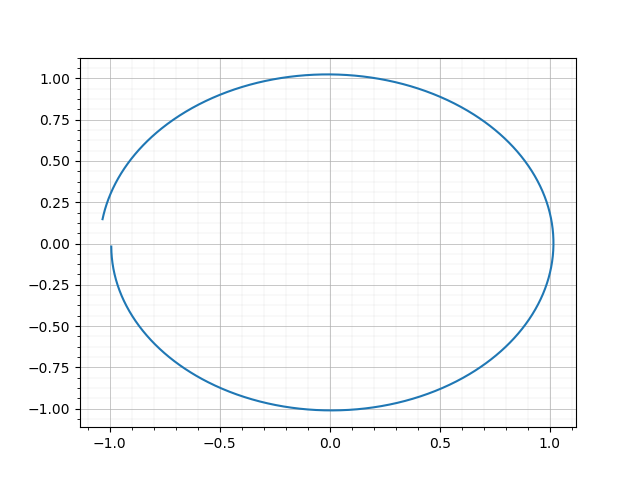
\includegraphics[scale=\scaleA]{binary_euler.png}
	\centering
	\caption{Normal Euler method: binary system}
	\label{fig:eulerbinary}
\end{figure}
Shown in figure \ref{fig:eulerbinary} is the result of the Euler method for the binary system. Due to numerical instability, the Earth's trajectory does not form a complete circle. Figure \ref{fig:eulermultiplanet} shows when the planets Mercury, Earth, Mars and Jupiter are modeled together, the numerical instability becoming even more apparent as something strange happens to Mercury. It is interesting to note the asymmetry of Mercury's death spiral.

\begin{figure}
	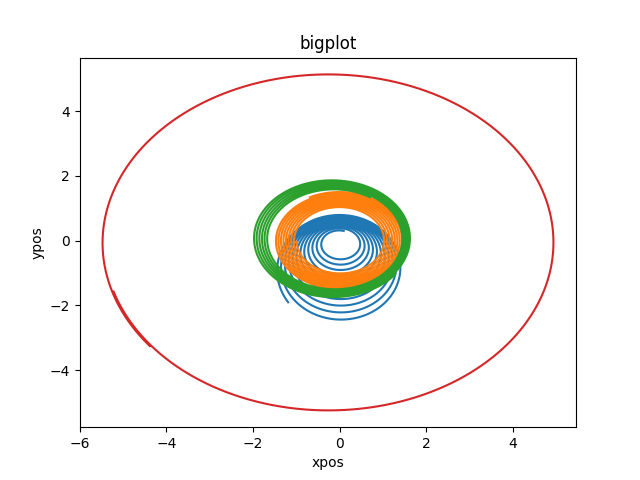
\includegraphics[scale=\scaleA]{euler_multiplanet.png}
	\centering
	\caption{Euler Method: four planet system}
	\label{fig:eulermultiplanet}
\end{figure}

The only reason those planets were chosen is because of geographical proximity, and to see the effect of a massive planet such as Jupiter. 

\subsection{Enhanced Euler}
The enhanced Euler method offers better numical stability leading to greater accuracy in the solution compared to the 'normal' Euler method.

\begin{figure}
	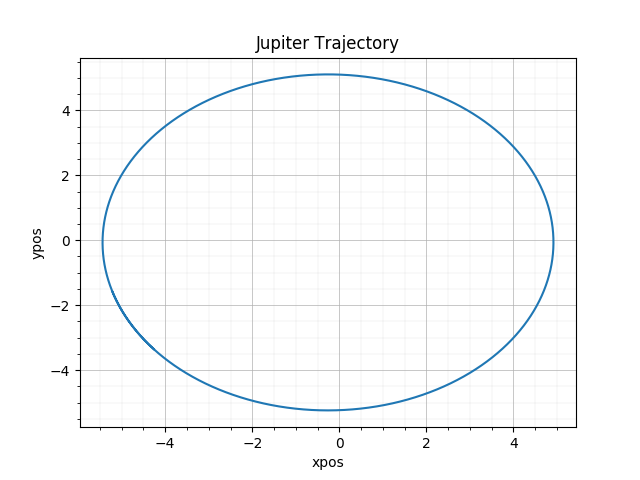
\includegraphics[scale=\scaleA]{euler_enhanced_jupiter.png}
	\centering
	\caption{Enhanced Euler Method: Jupiter alone}
	% TODO: Fix this, not really the same binary system
	\label{fig:enhancedeulerbinary}
\end{figure}

There is no visible gap here from numerical instability, however figure \ref{fig:enhancedeulermultiplanet} does show slight instability compared to the Verlet Method shown in figure \ref{fig:verletmultiplanet}.

\begin{figure}
	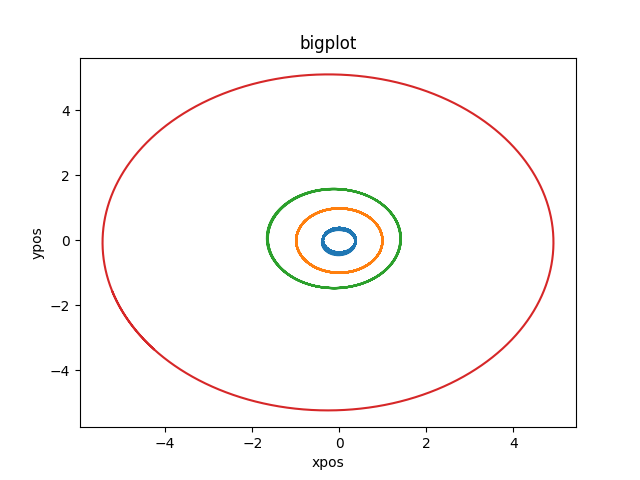
\includegraphics[scale=\scaleA]{euler_enhanced_multiplanet.png}
	\centering
	\caption{Enhanced Euler Method: four planet system}
	\label{fig:enhancedeulermultiplanet}
\end{figure}

\subsection{Velocity Verlet}
The Velocity Verlet solver shows the best numerical stability, leading to the best accuracy. While the enhanced Euler shows slight 'blurring' of the trajectories in figure \ref{fig:enhancedeulermultiplanet}, the Velocity Verlet solution in figure \ref{fig:verletmultiplanet} appears to contain perfect elipses.
\begin{figure}
	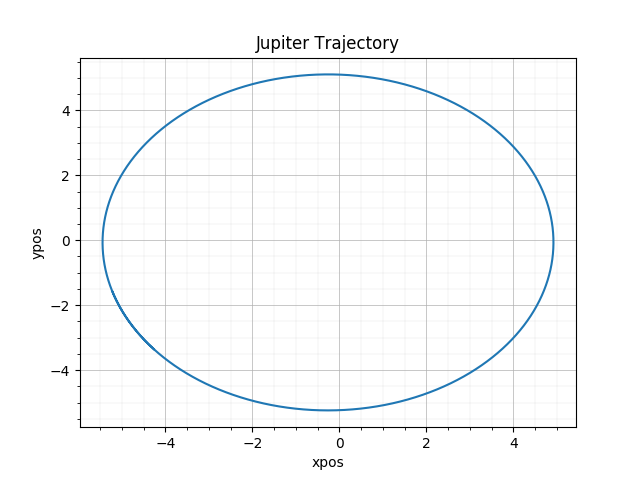
\includegraphics[scale=\scaleA]{verlet_jupiter.png}
	\centering
	\caption{Velocity Verlet: Jupiter alone}
	\label{fig:verletbinary}
\end{figure}

\begin{figure}
	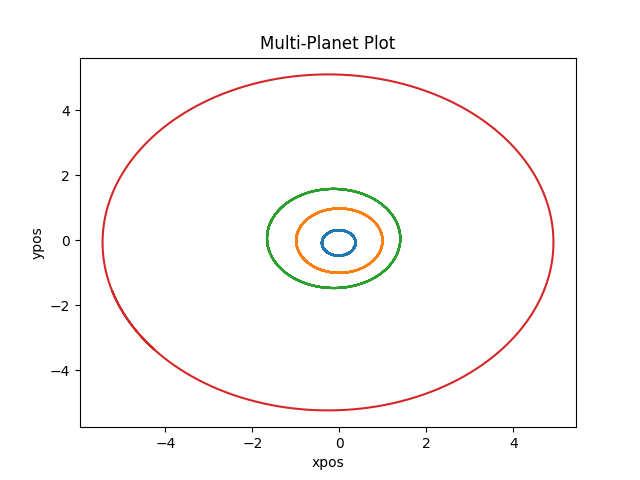
\includegraphics[scale=\scaleA]{verlet_multiplanet.png}
	\centering
	\caption{Velocity Verlet: four planet system}
	\label{fig:verletmultiplanet}
\end{figure}

\section{Conclusions and Future Work}
While the final presentation of all planets was not shown, due to the modularity of the code and the \texttt{Planet} class contained in \texttt{solarsystem.py}, the rest of the planets work just as well, but if all are plotted, then the middle ones are not clear.

Additionally, this code could be made to solve this in 3D space, and was structured such that the coordinates come last in a function (such as being returned by the planet difference function that computes distances between planets), to make adding the z axis as non-invasive as possible. Dare I might say trivial. Overall, this was an interesting project that really feels like something was 'built from scratch'. The process covered and skills learned were important, and it was nice to get experience with object orienting Python as 90\% of the use for it, especially as a replacement for Matlab in coursework seems to not require or benefit from using classes.
\end{document}
